\documentclass[letter,10pt]{article}
\usepackage[utf8]{inputenc}
\usepackage[spanish]{babel}
\usepackage{fancyvrb}
\usepackage{fancyhdr}
\usepackage{url}
\usepackage{verbatim}
\usepackage{graphicx}
\usepackage{rotating}
\usepackage{listings}
\usepackage{hyperref}

\parskip 1mm
\setlength{\topmargin}{0pt}
\oddsidemargin  0.5cm
\evensidemargin 0.5cm
\textwidth      15.5cm
\textheight     21.0cm
\headsep        4 mm
\parindent      0.5cm
\usepackage[scale=0.8]{geometry}
\usepackage[spanish]{babel}
\usepackage{float}


\pagestyle{fancyplain}

\lhead{Universidad Técnica Federico Santa María}
\rhead{Seminario de Arquitecturas de Sistemas Distribuidos}
\lfoot{}
\cfoot{}
\rfoot{\bf \thepage}
\renewcommand{\footrulewidth}{0.4pt}

\title{Propuesta de proyecto: Análisis de seguridad de Docker  }
\author{Maximiliano Osorio \\ mosorio@inf.utfsm.cl}
\date{Valparaíso, \today}
\newpage
\begin{document}
\maketitle

\newcommand{\container}{\textit{container}}
\newcommand{\containers}{\textit{containers}}

\section{Descripción del problema}
Como se vio en la propuesta, \textit{container-based virtualization} presenta mejor rendimiento que \textit{hypervisor-based virtualization} \cite{padala2007performance}, despliegue rapido de aplicaciones, portabilidad a través de host, control de versiones entre otras características\cite{Redhat:2015:Online}, pero las soluciones basadas en \textit{hypervisors} presentan un mejor aislamiento debido a que VM no puede comunicarse con el kernel de host, solo se puede comunicar con su mismo kernel. Por otra parte  \textit{container-based virtualization} necesita comunicarse con el kernel del host, por lo tanto permite que un atacante puede atacar al host u otro \container.\\ Este aspecto es importante de analizar para validar a \textit{container-based virtualization} como una solución en el producción en sistemas cloud u otro. 


\section{Trabajo realizado hasta la fecha}
\subsection{Investigación}
Al ser un tema nuevo y no conocido completamente por el autor ha sido necesario utilizar gran parte del tiempo en investigar y documentar como es el funcionamiento de Docker y las herramientas que utiliza para crear ambientes virtuales seguros. Es por ello que el marco teórico es extenso con el fin de poder diseñar posibles ataques y proponer soluciones o mitigaciones  a los ataques.
\subsubsection{Docker}
Docker es un proyecto open-source que utiliza la tecnología de los containers (libcontainer) para ``construir, migrar y correr aplicaciones distribuidas". Actualmente utilizado por Yelp, Spotify, entre otros \cite{Docker:2015:Online} \cite{marmolnetworking}
Docker es una solución que simplifica el uso de los \containers que han estado presente durante más de una década. Primero provee una interfaz simple y segura para crear y controlar \textit{containers} \cite{bui2015analysis}, segundo permite a los desarrolladores empaquetar y correr sus aplicaciones de manera sencilla y ademas se integra con herramientas terceras que permiten administración y despliegue como Puppet, Ansible y Vagrant. Además que existen diversas herramientas de orquestación como Mesos, Shipyard, Kubernetes, RancherOS y Docker Swarm. %todo: citar
  Docker puede separarse en dos grandes componentes: 
  
  	Dentro de Docker engine existen  componentes: 
	\begin{itemize}
		\item Docker Engine
		\item Docker Images
		\item Docker Containers
		\item Docker Registries
	\end{itemize}
	

Docker engine es una herramienta liviana y portable para manejar \textit{container-based virtualization} utilizando la arquitectura de la figura \label{fig:docker}. Los containers corren encima del servicio de Docker que se encarga de ejecutar y manejar los \containers. Docker Client, provee una interfaz para interactuar con los containers con los usuarios a través de RESTful APIs. \cite{bui2015analysis}\\

\begin{figure}[H]
  \centering
    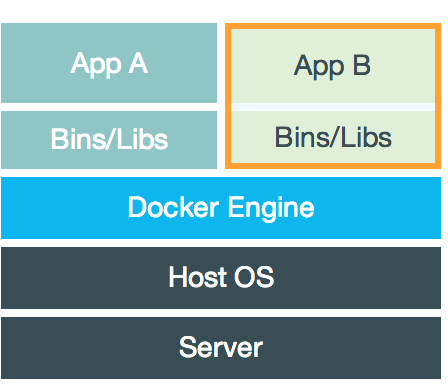
\includegraphics[width=0.3\textwidth]{images/docker.png}
    \caption{Docker}
    \label{fig:docker}
\end{figure}

	Docker utiliza una arquitectura de cliente-servidor, Docker Client habla con Docker daemon y este construye, maneja y corre los \textit{containers}. Docker Client y Docker daemon pueden correr en el mismo host o se puede conectar el cliente desde un host remoto. El cliente y el daemon se comunican en forma de sockets o RESTful API. \cite{Docker:2015:understanding}
	
\begin{figure}[H]
  \centering
    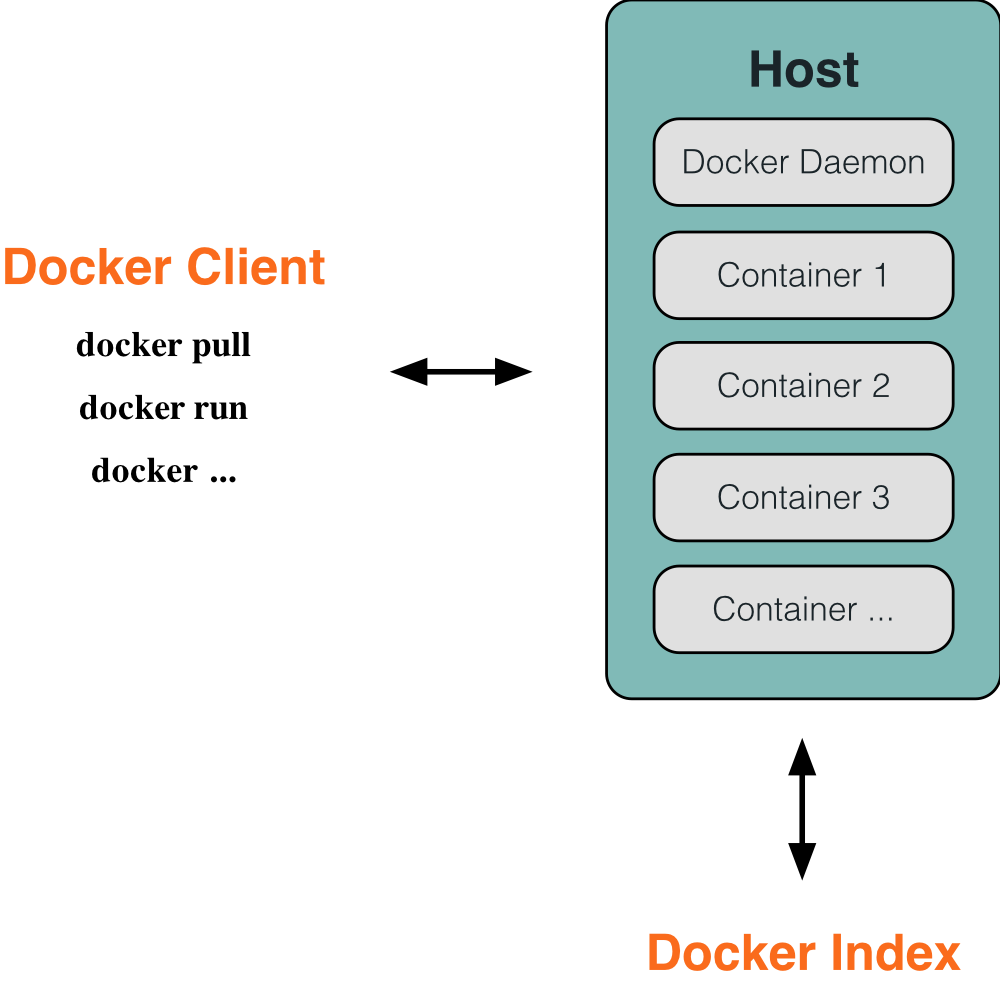
\includegraphics[width=0.3\textwidth]{images/architecture.png}
    \caption{Arquitectura}
    \label{fig:arquitectura}
\end{figure}	
	

	Una imagen de Docker (\textit{Docker Images}) es una plantilla de solo lectura \textit{read-only template}. Por ejemplo, una imagen puede contener un sistema operativo de Ubuntu con Apache y una aplicación web instalada o simplemente el sistema operativo. Las imágenes son usadas para construir \emph{Docker containers}. Cuando el usuario crea cambios en el \container, este cambio no ser realiza en la imagen. Docker añade una capa adicional con los cambios de la imagen. \cite{bui2015analysis} Por ejemplo, si el usuario utiliza una imagen base de Debian, luego añade el paquete emacs y luego añade el paquete apache, el estado de capas estaría representado por la figura \ref{fig:arquitectura} \cite{Docker:2015:Online}. Esto permite tener un proceso de distribución de imágenes más eficiente dado que solo es necesario distribuir las actualizaciones. \cite{bui2015analysis}. Lo \textit{filesystem} descrito anteriormente se denomina \textit{Union File System (UnionFS)}.
\begin{figure}[H]
  \centering
  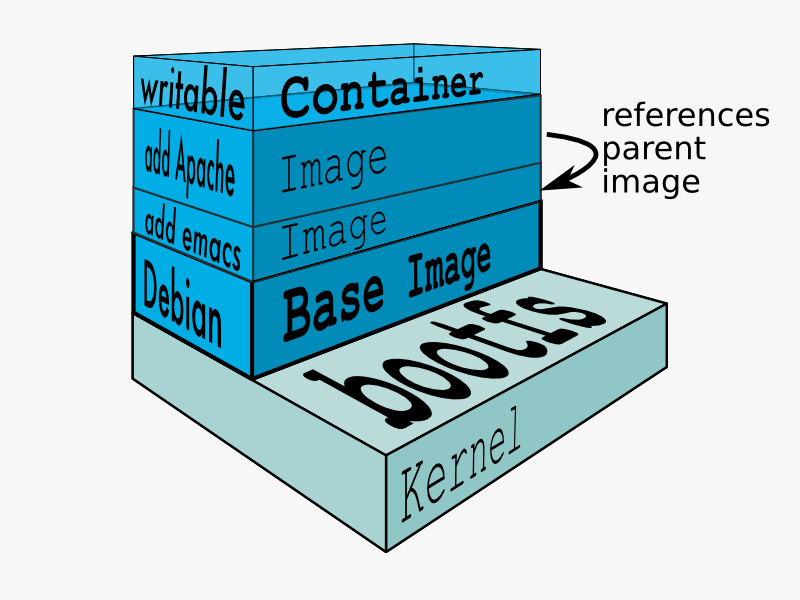
\includegraphics[width=0.6\textwidth]{images/docker-filesystems-multilayer}
    \caption{Representación \textit{union file system}}
    \label{fig:arquitectura}
\end{figure}	
	Docker \textit{Registries} son repositorios de imágenes estos pueden ser públicos y privados, vía a estos los usuarios pueden compartir las imágenes personalizadas o base. Docker cuenta con un repositorio publico llamado Docker Hub, Docker Hub es un repositorio central donde se pueden compartir y obtener imágenes, estas imágenes pueden ser verificadas tanto en la autenticidad y integridad a través un firmado y verificación de datos.\cite{bui2015analysis}. Los \textit{registries} son parte fundamental de eco sistema de Docker como una herramienta de desarrollo y despliegue de aplicaciones. Un caso de uso de un eco sistema típico que utiliza Docker está descrito por los siguientes eventos y la figura \ref{fig:dynamic}:
	\begin{itemize}
		\item Devs (desarrolladores) utiliza una imagen lista para usar ya sea por ejemplo Java, PHP o Rails, esta puede ser obtenida de repositorios públicos o privados.
		\item Paralelamente, ops (operaciones) pueden contribuir añadiendo patrones de seguridad o de despliegue.
		\item Devs y ops envían y traen sus cambios a través de Docker con comandos como commit, push, pull, tag hasta llegar a una versión de producción
		\item Ops traen los cambios a los servidores de producción, staging o quality assurance
		%todo: definir estas siglas
	\end{itemize}
	
\begin{figure}[H]
  \centering
  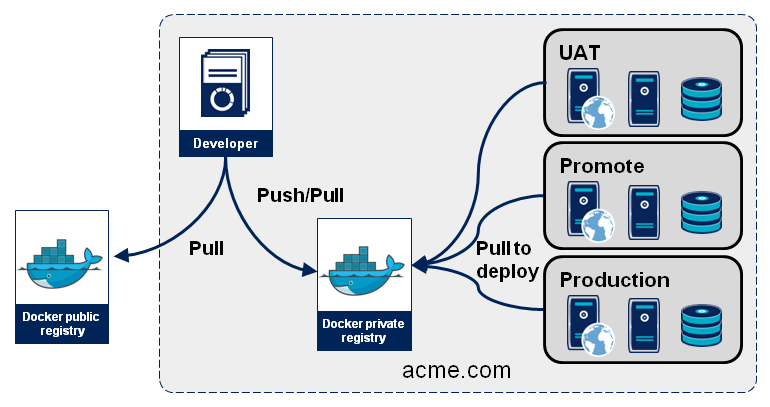
\includegraphics[width=0.6\textwidth]{images/registry-dynamic.png}
    \caption{Representación \textit{Dinámica de un \textit{Docker registry} }}
    \label{fig:dynamic}
\end{figure}	
	
Docker \textit{container} es un sistema operativo, con archivos de usuarios y metadata, como se mencionó anteriormente cada \textit{container} es construido a partir de una imagen. Esa imagen indica a Docker lo que contiene el \container, cual es proceso que debe correr cuando el  \textit{container} es creado y una variedad de configuraciones \cite{Docker:2015:understanding}. Para describir los pasos incluidos en la creación de un \emph{container}, se ejemplificará con la creación de uno.

\begin{verbatim}
	docker run -i -t ubuntu /bin/bash
\end{verbatim}
	\begin{itemize}
		\item \emph{Docker client} le informa al Docker que debe correr un \emph{container}.
		\item El comando será el \textit{init 0} del container en este caso en \emph{/bin/bash}
		\item \textbf{Traer la imagen:} Docker verifica la existencia de la imagen ubuntu y sino existe en el host, entonces Docker descarga de un \emph{registry} ya sea privado o publico. Si la imagen existe entonces crea el container.
		\item \textbf{Asignar un \emph{filesystem} y montar una capa \emph{read-write}:} El 
			\container es creado en el \emph{filesystem} y se añade una capa en modo 
			\emph{read-write}.
		\item \textbf{Asignar la red y el \emph{bridge interface}:} Crea la interfaz de red que permite que el Docker \container pueda hablar con el host.
		\item \textbf{Asignar un IP:} Asigna un ip del pool al \container
		\item \textbf{Capturar el \emph{output}, \emph{input} y errores}.
	\end{itemize}

Docker utiliza dos funcionalidades de Linux \emph{namespaces} y \emph{cgroups} para crear ambientes virtuales para los \containers. \emph{cgroups} o \emph{control groups} proveen un mecanismo de contabilidad y limites de recursos que pueden utilizar los \containers. \cite{bui2015analysis} Los \emph{namespaces} proveen del aislamiento que es llamado \container. Cuando sea crea un \container, Docker crea un conjunto de \emph{namespaces} para el \container. Los \emph{namespaces} utilizados por Docker: mount (mnt) para el manejo del montaje, pid para el aislamiento de los procesos, net para el manejo de interfaces y ipc para acceder a recursos de IPC. 
	Con el objetivo de detectar posibles brechas de seguridad se analizará cada una de esas.
	
	
	\subsubsection{Process isolation}
	
	Docker logra el aislamiento de los procesos separando los procesos en \emph{namespaces} y limitando los permisos y la visibilidad de los procesos a otros \emph{containers}. \emph{PID namespaces} (añadido en el kernel >= 2.6.3.2) es el mecanismo utilizado, logrando que un proceso que se encuentra en el \container solo pueda ver procesos que se encuentra en ese \container. Por lo tanto un atacante no puede observar procesos de otro \container, lo que hace difícil un ataque \cite{bui2015analysis} \cite{LVM:2015:Online}.
	
	\subsubsection{Filesystem isolation}
	
	Docker usa \emph{mount namespaces} o \emph{filesystem namespaces} para aislar los \emph{filesystems} asociados a los \containers. De la misma forma que ocurre con los procesos, los eventos del \emph{filesystem} que ocurre en el \container afectan a ese \container.
	Pero existen \emph{Linux kernel file systems} que deben ser montados desde host para que el \container pueda funcionar correctamente, esto permite a los \containers acceso directo al host. Docker utiliza dos técnicas para proteger el host: primero montar los \emph{file-systems} en modo lectura para evitar que puedan escribir en ellos y eliminar la opción de montar \emph{file-systems} en modo escritura y lectura. \cite{walsh:2014:Online}
	
	\subsubsection{Device isolation}
	Docker utiliza \emph{cgroups} que permite especificar que \emph{device} puede ser utilizado con el \container. Esto bloquea la posibilidad de crear y usar \emph{device nodes} que puedan ser utilizados para atacar el host. Los \emph{device nodes} que son creados para cada \container por defecto: son: /dev/console, /dev/null, /dev/zero, /dev/full, /dev/tty*, /dev/urandom, /dev/random, /dev/fuse \cite{walsh:2014:Online}
	
	\subsubsection{IPC isolation}
	IPC (\emph{inter-process communication} es un conjunto de objetos para el intercambio de data a través de los procesos, como semáforos, colas de mensajes, segmentos de memoria compartida. Los procesos corriendo en los \containers utilizan \emph{IPC namespaces} que permite la creación de un \emph{IPC} separado y independiente para cada \container, con esto se previene que procesos en un \container interfieran con otros \containers o el host.
	
		
	\subsubsection{Network isolation}
	Para cada \container, Docker crea una red independiente usnado \emph{network namespaces}, compuesta de su propia IP, rutas, \emph{network devices} Esto permite que el \container pueda interactuar con otro host a través de su propia interfaz.

	Por defecto, la conexión se realiza gracias al host que provee un \emph{Virtual Ethernet bridge} en la máquina host, llamado docker0 que automaticamente realiza un \emph{forward} de los paquetes entre las interfaces. Cuando Docker crea un nuevo \container, esto establece una interfaz de red virtual con un nombre único que se conecta con el \emph{bridge (docker0)} y con la interfaz \emph{eth0} del \container. \cite{bui2015analysis}
	
	\subsubsection{Limite de recursos}
	
	\emph{Cgroups} controlan la cantidad de recursos como CPU, memoria, \emph{disk I/O} que el \container puede utilizar. A partir de esto se protege contra ataques de DoS.

\subsection{Implementación}

Actualmente la implementación base se encuentra lista. Utilizando un nodo
Centos con project-atomic y Docker 1.5.0. Se habilitó SElinux para
realizar pruebas con un \emph{Mandatory Access Control}

\begin{verbatim}
Docker version 1.5.0, build a8a31ef/1.5.0
\end{verbatim}


\subsection{Discusión y posibles ataques}	

\subsubsection{Secure image repository}
Basado en la idea de Fernandez, Monge y Hashizume  de \emph{Secure
virtual machine image repository} \cite{fernandez_monge:2015} se investigó sobre si Docker hub cumple con los patrones especificados.  Fernandez, Monge y Hashizume definen defensas para un repositorio de VMI entre ellas se encuentran: Authenticator-Authorizer, Secure Channel, Security Logger/Auditor y filter \cite{fernandez_monge:2015}, basado en el changelog de Docker 1.3 se muestra que implementó un proceso de verificación de las imágenes llamado \emph{signed images} completando la lista de defensas nombradas,  Rudenberg \cite{rudenberg:2015:Online} y Jay \cite{jay:2014:Online} alertan que el proceso de traer un imagen no es seguro debido a que:
		\begin{itemize}
			\item Docker nunca verifica \emph{checksum} de la imagen permitiendo un ataque.
			\item Utilización de xz, escrito en C (un lenguaje \emph{memory-safe} potencialmente se podría ejecutar código malicioso y escalar en privilegios
		\end{itemize}
	Al probar realizar las pruebas, se determina que no afectan a la última versión de Docker.  Para más detalles consultar a CVE-2014-9356, CVE-2014-9357, CVE-2014-9358 \cite{lvm-cve:2014:Online}
\subsubsection{Network}

El modelo de red de Docker conecta la interfaz de \container con el 
\emph{bridge docker0} esto permite que exista comunicación de layer-2 entre 
los \containers y el host. Actualmente un \container es capaz de comunicarse
con otro \container por defecto en Docker, en caso de querer aislar un 
\container se debe utilizar la opción --icc. En este caso no es útil debido que 
a la opción --icc actua a nivel de iptables o sea \emph{layer 3} y los 
\containers están conectados por \emph{layer 2} por lo tanto es posible realizar 
un ARP-spoofing. nyatec propone dos soluciones para esto: eliminar la capacidad 
de NET\_RAW para evitar que el \container puede crear \emph{PF\_PACKET sockets} 
que son necesarios para el ARP spoofing attack o la utilización de etables para 
filtrar los \emph{Ethernet frame} con direcciones de destino incorrecto. \cite{nyantec:2015:Online}.

\textbf{Prueba de concepto}:  Se crean dos \containers, la imagen de atacante contiene las programa arpspoof. 
\begin{verbatim}
	docker run --name=atacante -ti ubuntu_arp bash
	docker run --name=victima --ti ubuntu bash
\end{verbatim}

El atacante hace arp-spoofing, a la victima (172.17.0.3)
\begin{verbatim}
	for i in $(seq 1 5); do  arpspoof -t 172.17.0.3 172.17.42.1 > /dev/null 2>&1 &; done;
\end{verbatim}
Y la victima sufre el ataque
\begin{verbatim}
? (172.17.0.4) at 02:42:ac:11:00:04 [ether] on eth0
? (172.17.42.1) at 02:42:ac:11:00:04 [ether] on eth0
\end{verbatim}



\section{Trabajo restante}

\begin{itemize}
	\item Completar investigación con \emph{Linux Capabilities} y \emph{Mandatory Access Control}
	\item Alcances de ataques en un ambiente de Docker con SElinux (MAC) integrado.
	\item Es posible asegurar el host o los \containers   si el atacante salió del \container.
\end{itemize}

\section{Conclusiones preliminares}
Docker es un sistema seguro siendo utilizado con la configuración por defecto aunque si existen vulnerabilidades como se nombro. La utilización de herramientas complementarías como SElinux aumentan el grado de seguridad es por ello que en la siguiente entrega el informe se centrará en la utilización de Docker con SElinux y resolver la pregunta ¿podemos asegurar el host u otros \containers si el atacante escapó del \container?


\bibliographystyle{plain}
\bibliography{Referencias}

\end{document} 